\documentclass{article}
\usepackage[spanish]{babel}
\usepackage{graphicx}
\usepackage{subfigure}
\usepackage{amsmath}
\usepackage{hyperref}  % hyperlinks
\graphicspath{{/home/vian/0_uam/1_TFG/latex/img/}}

\title{integracion, pruebas y resultados}

\begin{document}

\maketitle{}
\tableofcontents{}

\newpage

En las ejecuciones de QAOA, con el fin de medir la eficacia de los resultados obtenidos entre métricas distintas, se han realizado los siguientes tipos de pruebas:
\begin{itemize}
\item \textbf{Estadística máxima:}
  Con este método se busca obviar el ruido presente en cada ejecución. Para ello se realizan \textit{n} iteraciones distintas sobre el algoritmo y para cada una de ellas:
  \begin{enumerate}
  \item
    Se ejecuta el optimizador clásico para hallar los parámetros óptimos (esto supone la ejecución del circuito cuántico el número de veces necesario para que el optimizador encuentre un mínimo local).
  \item
    Se ejecuta el circuito una vez más con los parámetros óptimos.
  \item \label{it:5-definicion_estadistica_max}
    Se obtiene el camino dado por el algoritmo para recorrer el grafo y se añade dicho camino a un diccionario para su posterior revisión. En el caso de la figura \ref{fig:5-primer_grafo/sin_restriccion_extra/primer_paper_aer_resultado}
    el resultado sería \textit{10101}, es decir, el camino con mayor valor.
  \end{enumerate}
  
\item \textbf{Estadística global:}
  A diferencia de la estrategia previamente explicada, al realizar el paso \ref{it:5-definicion_estadistica_max} se toman todos los caminos resultantes de la ejecución del circuito con los parámetros \(\beta_{opt}\) y \(\gamma_{opt}\).
  De esta forma, una ejecución como la dada en la figura \ref{fig:5-primer_grafo/sin_restriccion_extra/primer_paper_aer_resultado}
  se ve condicionada por todos los resultados, no únicamente por el camino con valor máximo.
  
\item \textbf{Función gamma:}
  Se ha utilizado para comprobar la forma general que tiene la función \textit{execute\_circuit}, a minimizar por el optimizador clásico. Para ello se han realizado circuitos de una sola capa y se ha mantenido el parámetro \(\beta=1\). Se ha decidido así porque dicho parámetro se encarga del ángulo de rotación de los operadores \(\sigma_{x}\), de construcción trivial en comparación con los operadores dependientes de \(\gamma\).
  % TODO: Referenciar punto del apéndice donde se hable sobre la construcción de las puertas Rx y Rz
  Al variar \(\gamma\) y graficar la función resultante se puede intuir la probabilidad de encontrar mínimos locales en lugar del mínimo global. Esto se traduce como la posibilidad de encontrar un resultado subóptimo para el problema, es decir, que el algoritmo falle.
\end{itemize}

A continuación se mostrarán los resultados de ejecución utilizando ambos paradigmas, esto es, QAOA y Quantum Annealing, además de explorar el rendimiento de las ejecuciones en Qiskit variando los métodos para construir la función de coste.

% TODOOOO: Los resultados en general están demasiado mal. Sigo con Zhiqiang y luego veo qué se hace aquí. Los modificadores originales (correctos "teóricamente") dan una función gamma muy extraña, con muchos "baches"
\section{Primer grafo}

\begin{figure}[htbp]
  \centering
  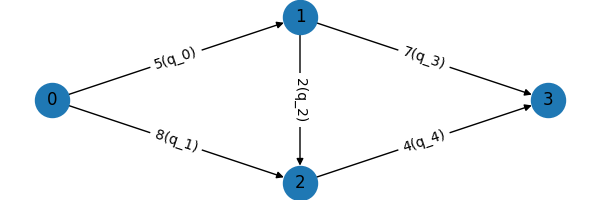
\includegraphics[scale=0.75]{primer_grafo/primer_grafo}
  \caption{Primer grafo. Artículo \cite{multi-objective_routing_optimization}}
\end{figure}

\subsection{Resultados de Qiskit}

\subsubsection{Solución del artículo}
\label{sec:5-primer-paper-resultados_qiskit}
En las siguientes muestras se ha buscado replicar los resultados del artículo. Esto ha sido probado ya que, empleando los parámetros \(\beta = 0.28517317\) y \(\gamma = -5.05969577 \) dados como óptimos, se obtiene un gráfico muy similar al dado: \\

\begin{figure}[htbp]
  \centering
  \subfigure[Resultado del artículo]{
    \includegraphics[width=0.44\textwidth]{primer_grafo/sin_restriccion_extra/primer_paper_orig_resultado}
  }
  \subfigure[Resultado obtenido]{
    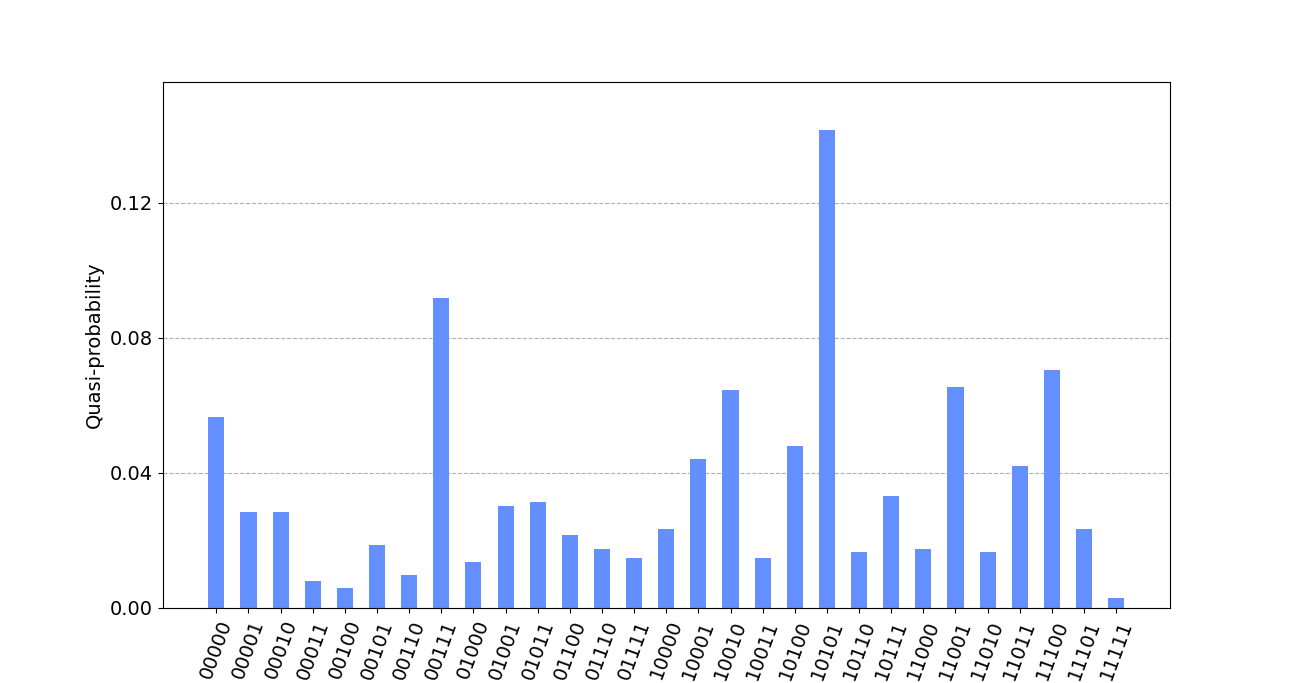
\includegraphics[width=0.51\textwidth]{primer_grafo/sin_restriccion_extra/primer_paper_aer_resultado}
  }
  \caption{} \label{fig:5-primer_grafo/sin_restriccion_extra/primer_paper_aer_resultado}
\end{figure}

De esta forma, se tiene que los resultados del artículo deberían ser equivalentes a los obtenidos en esta instancia del algoritmo.

\begin{table}[htbp]
  \centering
  \begin{tabular}{|c|r|r|}
    \hline
    \textbf{nº Capas} & \textbf{Estadística máxima (\%)} & \textbf{Estadística global (\%)} \\ \hline
    p = 1 & 91.3\% & 39.34\% \\ \hline
    p = 2 & 64.6\% & 24.16\% \\ \hline
    p = 3 & 63.4\% & 18.82\% \\ \hline
    p = 4 &  9.4\% &  5.38\% \\ \hline
    p = 5 & 67.9\% & 19.45\% \\ \hline
    p = 6 & 29.8\% & 12.59\% \\ \hline
    p = 7 & 28.9\% &  9.12\% \\ \hline
    p = 8 & 36.7\% & 12.49\% \\ \hline
  \end{tabular}
  \caption{Resultados de la ejecución de la versión de QAOA del artículo}
  \label{tab:5-primer-paper-aer_estadisticas}
\end{table}

El primer resultado a resaltar en la tabla \ref{tab:5-primer-paper-aer_estadisticas} es un empeoramiento de los resultados a medida que se aumenta el número de capas, lo cual es contrario a lo esperado teóricamente. \\
% FIXMEEEE: Esto tiene que estar mal, lo muestro de todas formas? (el hecho de que al aumentar p empeore el algoritmo)
Además, la gran diferencia entre los resultados dados por la estadística máxima y la estadística global denotan una gran cantidad de ruido al ejecutar el algoritmo, lo cual se corrobora viendo los resultados de ejecuciones concretas, como los dados en la figura \ref{fig:5-primer_grafo/sin_restriccion_extra/primer_paper_aer_resultado}. \\

El resultado de la función gamma es el siguiente:
\begin{figure}[htbp]
  \centering
  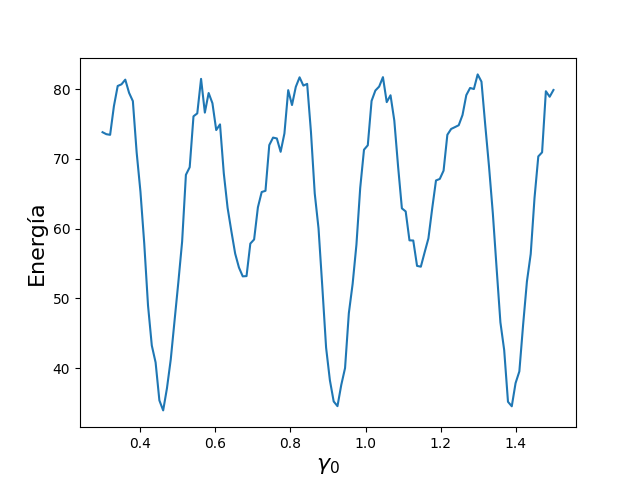
\includegraphics[scale=0.5]{primer_grafo/sin_restriccion_extra/primer_paper_p_27_gamma_fun}
  \caption{Función gamma. Caso del artículo} \label{fig:5-primer_grafo/sin_restriccion_extra/primer_paper_p_27_gamma_fun}
\end{figure}

Se puede ver que existen un gran número de mínimos locales, lo cual dificulta la tarea del optimizador clásico. Esto se corrobora ya que, al inicializar los parámetros como \(\beta = 1.0 \ \gamma = 0.5\), para \(p = 1\) se obtiene el camino óptimo el 100\% de las ejecuciones. \\
% TODO: Comparar esta función gamma con la que aparece en MAX-CUT, esto estará en el anexo
Este proceso de inicializar los parámetros con valores concretos no sería una solución válida, ya que se trata de una metodología no automática en la que, para ejecutar correctamente el algoritmo, se necesitaría conocer antes su propio resultado. Además la ejecución correcta sucede para \(p = 1\), pero al igual que el caso por defecto (\(\beta = 1.0 \ \gamma = 1.0\)), no escala correctamente al aumentar el número de capas.

\subsubsection{Modificaciones a la solución del artículo}
Partiendo de la solución del artículo descrita en la sección \ref{sec:5-primer-paper-resultados_qiskit}, se han realizado cambios a la función de coste y a la construcción del circuito cuántico con el fin de encontrar el mejor resultado. Esto se ha realizado para poder comparar el rendimiento de la mejor solución encontrada con el rendimiento del algoritmo de Quantum Annealing de D-Wave.

Las modificaciones empleadas han sido las siguientes:

\paragraph{Modificadores originales}
Al construir el circuito cuántico, utilizar para los operadores lineales los ángulos obtenidos teóricamente, en lugar de los vistos en el artículo. \\
Las estadísticas obtenidas en la \textit{tabla \ref{tab:5-primer-mod_originales-aer_estadisticas} } no dan ningún resultado positivo. Se aprecia un comportamiento similar al visto en los resultados del tercer grafo, en la \textit{tabla \ref{tab:5-zhiqiang-aer_estadisticas} } en cuanto a que se mejoran las estadísticas hasta las 3 capas y luego disminuyen.
% TODOO: ¿Explicar la diferencia en los modificadores? Hay que explicarlo
\begin{table}[htbp]
  \centering
  \begin{tabular}{|c|r|r|}
    \hline
    \textbf{nº Capas} & \textbf{Estadística máxima (\%)} & \textbf{Estadística global (\%)} \\ \hline
    p = 1 &  0.5\% &  4.05\% \\ \hline
    p = 2 &  9.2\% &  5.83\% \\ \hline
    p = 3 & 54.8\% & 12.98\% \\ \hline
    p = 4 & 11.1\% &  7.00\% \\ \hline
    p = 5 &    6\% &  5.71\% \\ \hline
  \end{tabular}
  \caption{Resultados de la ejecución de QAOA utilizando los ángulos obtenidos teóricamente}
  \label{tab:5-primer-mod_originales-aer_estadisticas}
\end{table}

La función gamma resultante se muestra en la \textit{figura \ref{fig:5-primer-mod_originales-gamma_fun}}. Tiene un mínimo global menos claro con respecto a la función gamma de la versión del grafo del paper, en la \textit{figura \ref{fig:5-primer_grafo/sin_restriccion_extra/primer_paper_p_27_gamma_fun}}. Además a diferencia de dicha gráfica, en esta no se aprecia periodicidad alguna.
\begin{figure}[htbp]
  \centering
  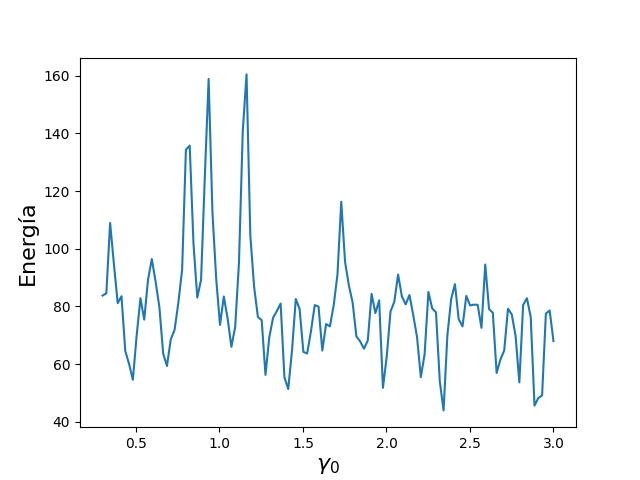
\includegraphics[scale=0.5]{primer_grafo/sin_restriccion_extra/primer-paper-mod_originales-gamma_fun}
  \caption{Función gamma. Con modificadores originales.}
  \label{fig:5-primer-mod_originales-gamma_fun}
\end{figure}

\paragraph{P=40}
% TODOOO: Repetir estas ejecuciones y hacer función gamma, por ahora salen demasiado mal como para mostrarlas
Incrementar el valor del parámetro P (correspondiente al modificador de Lagrange)
% TODO: Citar multiplicador de lagrange del anexo
al construir la función de coste, para así aumentar la penalización en caso de fallo.

\paragraph{Restricción extra}
Añadir una restricción a la función de coste, que especifique que solo se puede acceder al último nodo por una de las aristas que lleguen a este.
% TODOO: Esto seguramente no se explique aquí, en algún sitio hablar sobre la restricción extra. SI SE QUITA LA FORMULA QUITARLA DE LA CITA DE LA TABLA DE ABAJO
\begin{equation}
  \label{eq:5-primer-restriccion_extra}
  X_{13} + X_{23} = 1
\end{equation}

% TODOOO: Añadir estadísticas globales y repetir estadísticas máximas, tal vez con más capas tb
\begin{table}[htbp]
  \centering
  \begin{tabular}{|c|r|r|}
    \hline
    \textbf{nº Capas} & \textbf{Estadística máxima (\%)} & \textbf{Estadística global (\%)} \\ \hline
    p = 1 & 93.8\% & 37.83\% \\ \hline
    p = 2 & 64.6\% & 26.16\% \\ \hline
    p = 3 & 84.8\% & 27.82\% \\ \hline
    p = 4 & 56.0\% & 23.47\% \\ \hline
    p = 5 & 88.1\% & 46.40\% \\ \hline
    p = 6 & 88.1\% & 21.83\% \\ \hline
  \end{tabular}
  \caption{Resultados de la ejecución de QAOA añadiendo la restricción de la fórmula \ref{eq:5-primer-restriccion_extra}}
  \label{tab:5-primer-restriccion_extra-aer_estadisticas}
\end{table}

Los resultados (\textit{tabla \ref{tab:5-primer-restriccion_extra-aer_estadisticas}}) presentan una ligera mejora con respecto a los presentes en la \textit{tabla \ref{tab:5-primer-paper-aer_estadisticas}}, tanto para las estadísticas máximas como globales. \\

La función gamma resultante (\textit{figura \ref{fig:5-primer_grafo/con_restriccion_extra/primer_restr_aer_gamma_fun}}) toma, en comparación con la original (\textit{figura \ref{fig:5-primer_grafo/sin_restriccion_extra/primer_paper_p_27_gamma_fun}}), unos valores elevados. Se distingue un incremento en la diferencia entre los mínimos globales y los mínimos locales (no globales).
\begin{figure}[htbp]
  \centering
  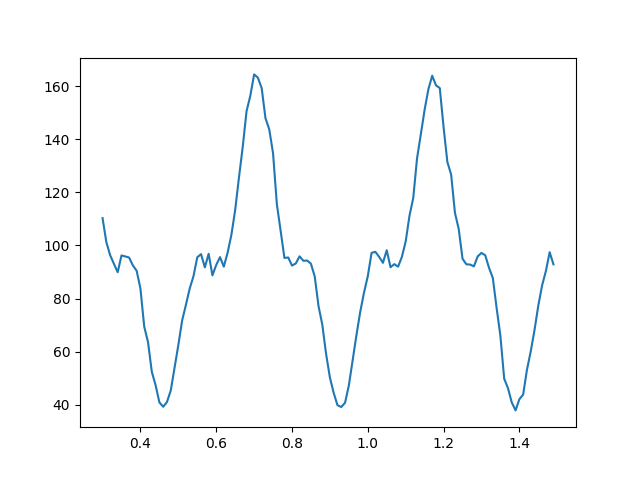
\includegraphics[scale=0.5]{primer_grafo/con_restriccion_extra/primer_restr_aer_gamma_fun}
  \caption{Función gamma. Con restricción extra}
  \label{fig:5-primer_grafo/con_restriccion_extra/primer_restr_aer_gamma_fun}
\end{figure}
\subsection{Resultados en ordenador cuántico real}
Utilizando la herramienta Runtime de Qiskit se han realizado ejecuciones del código para comprobar sus resultados en ordenadores reales.

El funcionamiento ha sido obtener los parámetros \(\alpha\) y \(\beta\) en dichos ordenadores y después ejecutar una vez más en un simulador para obtener el resultado al problema.
\subsubsection{\(p = 1\)}
El código ha sido ejecutando con el error encontrado en el artículo, tratando así de asemejarse a los resultados obtenidos en el mismo.

El resultado obtenido ha sido el siguiente:
\begin{verbatim}
 message: Optimization terminated successfully.
 success: True
  status: 1
     fun: 52.81120901157566
       x: [ 7.624e-01  4.636e-01]
    nfev: 30
   maxcv: 0.0
\end{verbatim}
Este mensaje es devuelto por el optimizador clásico \href{https://docs.scipy.org/doc/scipy/reference/generated/scipy.optimize.minimize.html}{scipy.optimize.minimize} y significa que se han encontrado los parámetros \(\alpha = 0.7624 \text{ y } \beta = 0.4636\), con los que la función \textit{execute\_circuit} devuelve un valor de 52.81. Esto está muy lejos de ser una media óptima, ya que esto se daría al obtener en todos los casos el camino más corto, lo que daría una media de 11 (el coste de dicho resultado).

El otro valor a remarcar, \textit{nfev=30}, se refiere al número de ejecuciones de la función \textit{execute\_circuit} realizadas.

Los parámetros obtenidos, ejecutados en un simulador, dan el siguiente resultado:
\begin{figure}[htbp]
  \centering
  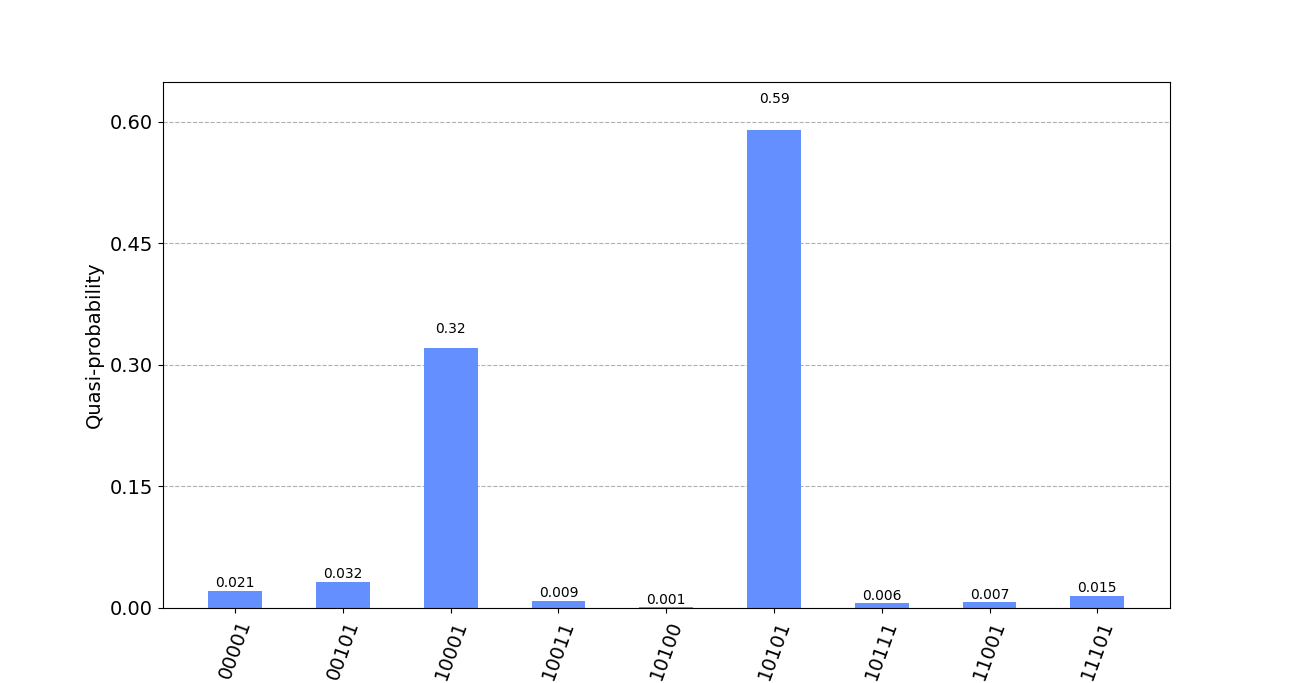
\includegraphics[scale=0.4]{primer_grafo/sin_restriccion_extra/primer-runtime-mod_paper-1_capa-nairobi_aer}
  \caption{Ejecución de \(\alpha, \beta\) en simulador}
  \label{fig:5-primer_grafo/sin_restriccion_extra/primer-runtime-mod_paper-1_capa-nairobi_aer}
\end{figure}

Esto indica que el motivo de obtener un resultado inesperadamente alto de la función se debe a la presencia de un camino, \textit{10001}, de coste elevado obtenido un gran número de veces. Este camino es costoso, con valor de 63, debido a que rompe varias restricciones de la función de coste.

Estos mismos parámetros resultados de la ejecución en \textit{ibm\_nairobi} han sido ejecutados en el ordenador de \textit{ibm\_lagos}, dando los resultados de la figura \ref{fig:5-primer_grafo/sin_restriccion_extra/primer-runtime-mod_paper-1_capa-nairobi_lagos}.
\begin{figure}[htbp]
  \centering
  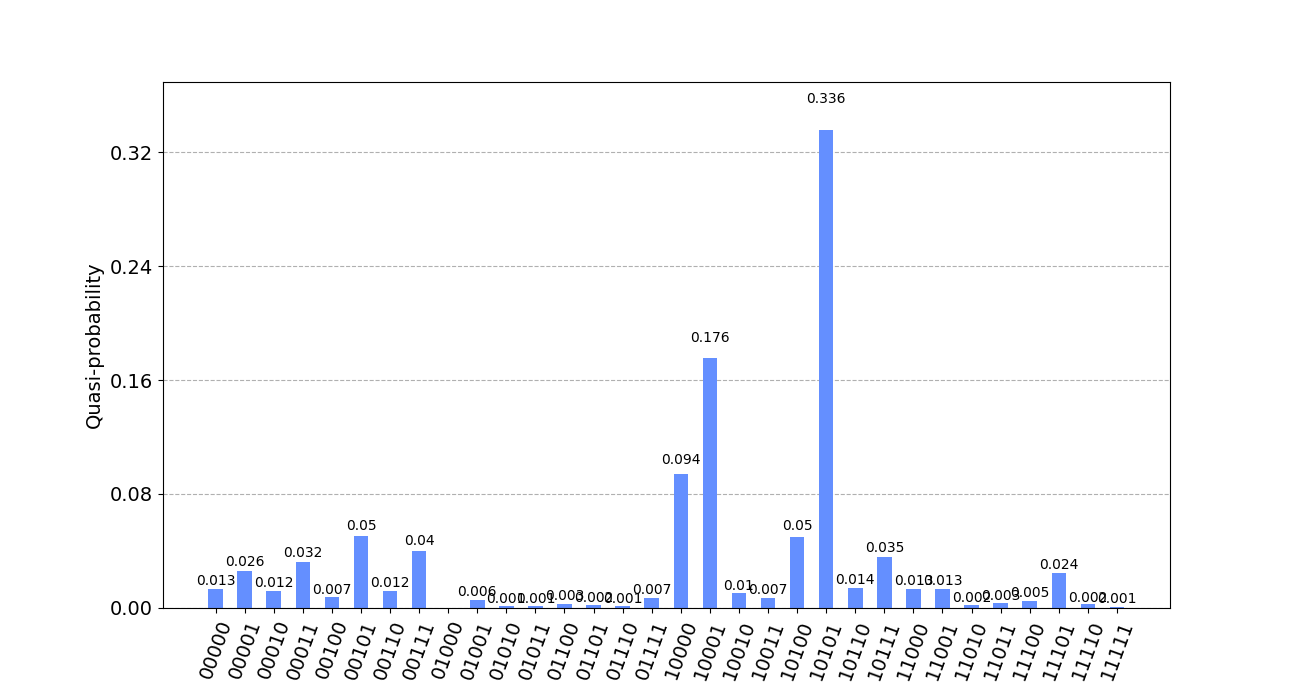
\includegraphics[scale=0.4]{primer_grafo/sin_restriccion_extra/primer-runtime-mod_paper-1_capa-nairobi_lagos}
  \caption{Ejecución de \(\alpha, \beta\) en \textit{ibm\_lagos}}
  \label{fig:5-primer_grafo/sin_restriccion_extra/primer-runtime-mod_paper-1_capa-nairobi_lagos}
\end{figure}

Comparando las imágenes
\ref{fig:5-primer_grafo/sin_restriccion_extra/primer-runtime-mod_paper-1_capa-nairobi_aer}
y \ref{fig:5-primer_grafo/sin_restriccion_extra/primer-runtime-mod_paper-1_capa-nairobi_lagos}
se aprecia la diferencia de ejecutar unos mismos parámetros en un simulador y un ordenador cuántico real. Aunque los resultados sean similares el número de ocurrencias de la cadena de bits correspondiente con el camino óptimo disminuye notablemente en la ejecución real, debido al ruido presente en toda ejecución de un circuito cuántico.

\newpage


\subsection{Resultados de D-Wave}
Con respecto a los resultados de aplicar Quantum Annealing utilizando los sistemas de D-Wave se ha obtenido el resultado de la tabla \ref{tab:5-primer-dwave_estadisticas}

\begin{table}[htbp]
  \centering
  \begin{tabular}{|c|r|r|}
    \hline
    \textbf{Camino} & \textbf{Energía} & \textbf{Número de ocurrencias} \\ \hline
    10101 (\textbf{Óptimo}) & 11 & 348 \\ \hline
    10010                   & 12 & 373 \\ \hline
    01001                   & 12 & 294 \\ \hline
    00000                   & 54 &   4 \\ \hline
    10000                   & 58 &   1 \\ \hline
    00001                   & 59 &   1 \\ \hline
    10100                   & 60 &   1 \\ \hline
    00101                   & 61 &   1 \\ \hline
    01010                   & 69 &   1 \\ \hline
  \end{tabular}
  \caption{Resultados de la ejecución del primer grafo en D-Wave}
  \label{tab:5-primer-dwave_estadisticas}
\end{table}

La energía se refiere al coste de dicho camino de acuerdo con la función de coste utilizada. Se puede ver cómo, aunque se encuentre el camino óptimo un menor número de veces que en QAOA, existe una mayor coherencia en los resultados. Esto es así porque los caminos con mayores ocurrencias son los que tienen menor energía, mientras en las ejecuciones de Qiskit se pueden ver ejemplos, como es el camino 00111 en la figura \ref{fig:5-primer_grafo/sin_restriccion_extra/primer_paper_aer_resultado} con un gran número de ocurrencias pero también una energía elevada.
\footnote{En la ejecución de Qiskit, la energía del camino ``00111'' es 150. Esto se debe a que se rompen varias restricciones presentes en la función de coste. Este valor puede variar dependiendo del multiplicador de Lagrange empleado
  % TODO: Citar multiplicador de lagrange del anexo
  y las restricciones utilizadas.}

\section{Tercer grafo}

\begin{figure}[htbp]
  \centering
  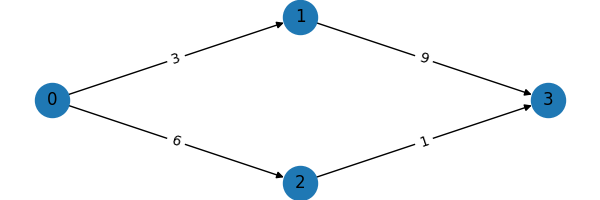
\includegraphics[scale=0.75]{zhiqiang_grafo/zhiqiang_grafo}
  \caption{Tercer grafo. Artículo \cite{solving_shortest_path_with_qaoa}}
\end{figure}

\subsection{Resultados de Qiskit}
\begin{table}[htbp]
  \centering
  \begin{tabular}{|c|r|r|}
    \hline
    \textbf{nº Capas} & \textbf{Estadística máxima (\%)} & \textbf{Estadística global (\%)} \\ \hline
    p = 1 &  0.6\% &  5.9\% \\ \hline
    p = 2 & 30.7\% & 16.9\% \\ \hline
    p = 3 & 93.8\% & 26.0\% \\ \hline
    p = 4 & 66.9\% & 39.4\% \\ \hline  % EL OTRO MAX RESULTADO OBTENIDO (0101 - 33.1%) ES EL SEGUNDO VALIDO, ESO ES POCO COMÚM
    p = 5 &  1.6\% & 15.0\% \\ \hline  % EL OTRO MAX RESULTADO OBTENIDO (0101 - 98.4%) ES EL SEGUNDO VALIDO, ESO ES POCO COMÚM. El global resultado es 0101 con un 55.17%
    p = 6 & 81.0\% & 32.9\% \\ \hline
    p = 7 & 36.5\% & 26.4\% \\ \hline
    p = 8 & 64.2\% & 32.8\% \\ \hline
  \end{tabular}
  \caption{Resultados de la ejecución de QAOA del tercer grafo. P=20. Modificadores del paper (omitir \(2*\gamma\))}
  \label{tab:5-zhiqiang-aer_estadisticas}
\end{table}

A diferencia de las ejecuciones del primer grafo (tabla \ref{tab:5-primer-paper-aer_estadisticas}), aquí se ve una clara mejora con el aumento del número de capas.

Además, para el caso \(p = 3\) se aprecia una distancia mucho mayor a la habitual entre la estadística máxima y global. A efectos prácticos se toma como medida de fiabilidad la estadística máxima, ya que significa que se ha encontrado el camino óptimo el 93.8\% de las ejecuciones realizadas.

El resultado de la función gamma es el siguiente:
\begin{figure}[htbp]
  \centering
  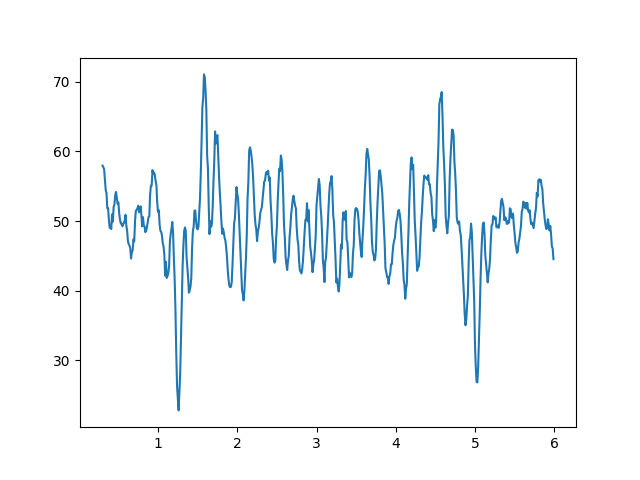
\includegraphics[scale=0.5]{zhiqiang_grafo/modificadores_paper/zhiqiang_p_20_gamma_fun}
  \caption{Función gamma del tercer grafo. P=20}
\end{figure}
A diferencia de las funciones gamma del grafo para el problema de MAX-CUT y el primer grafo de QAOA, en esta gráfica se ve mucho más ruido.

Esto se compara también con la gráfica resultante de ejecutar este mismo problema utilizando, para los operadores lineales del circuito, los ángulos obtenidos teóricamente (en lugar de basarse en los obtenidos del artículo).
% TODOOOOO: Insertar gamma function con modificadores originales y citarla aquí
% TODOO: ¿Explicar la diferencia en los modificadores? Hay que explicarlo

\begin{table}[htbp]
  \centering
  \begin{tabular}{|c|r|r|}
    \hline
    \textbf{nº Capas} & \textbf{Estadística máxima (\%)} & \textbf{Estadística global (\%)} \\ \hline
    p = 1 &  0.1\% &  9.79\% \\ \hline
    p = 2 & 10.0\% & 20.20\% \\ \hline
    p = 3 & 38.1\% & 19.47\% \\ \hline
    p = 4 &  0.7\% & 27.33\% \\ \hline  % el 99.3\% de resultados ha sido 0101 (en lugar de 1010)
    p = 5 & 40.6\% & 24.29\% \\ \hline
    p = 6 & 30.7\% & 29.29\% \\ \hline
    p = 7 & 49.3\% & 24.60\% \\ \hline
    p = 8 & 71.4\% & 36.34\% \\ \hline
  \end{tabular}
  \caption{Resultados de la ejecución de QAOA del tercer grafo. Ángulos teóricos}
\end{table}

% FIXMEEEEEE: Tal vez quitar? No es significativo. Si se queda comentar la tabla.
\begin{table}[htbp]
  \centering
  \begin{tabular}{|c|r|r|}
    \hline
    \textbf{nº Capas} & \textbf{Estadística máxima (\%)} & \textbf{Estadística global (\%)} \\ \hline
    p = 1 &    0\% &  7.43\% \\ \hline
    p = 2 & 40.3\% & 14.69\% \\ \hline
    p = 3 & 62.0\% &  21.9\% \\ \hline
  \end{tabular}
  \caption{Resultados de la ejecución de QAOA del tercer grafo. P=40}
\end{table}

\subsection{Resultados de D-Wave}
\begin{table}[htbp]
  \centering
  \begin{tabular}{|c|r|r|}
    \hline
    \textbf{Camino} & \textbf{Energía} & \textbf{Número de ocurrencias} \\ \hline
    1010 (\textbf{Óptimo}) &  7 & 776 \\ \hline
    0101                   & 12 & 247 \\ \hline
    0010                   & 46 &   1 \\ \hline
  \end{tabular}
  \caption{Resultados de la ejecución del tercer grafo en D-Wave}
\end{table}

Al igual que en anteriores ejecuciones utilizando Quantum Annealing, se mantiene la coherencia en los resultados. El resultado más producido es el camino óptimo, mientras que el segundo camino más producido es el otro único camino válido (sin romper ninguna restricción).

\bibliographystyle{abbrv}
\bibliography{bibliografia}

\end{document}

%%% Local Variables:
%%% mode: latex
%%% TeX-master: t
%%% End:
